\documentclass[11pt, a4paper]{article}
%\usepackage{proj1}
\usepackage{natbib}
\usepackage{fancyhdr}  
\usepackage{subcaption}
\usepackage{caption}
\usepackage{graphicx}
\usepackage[autolanguage,nosepfour]{numprint}
\usepackage{multirow}
\linespread{1.25} 
\setlength{\parindent}{0cm}
\graphicspath{{Images/}}
\usepackage{hyperref}
\usepackage{amsmath}
\usepackage{amsfonts}
\usepackage{amssymb}
\usepackage{amsthm}
\usepackage{mathtools}
\usepackage{commath}
\usepackage{bbm}
\usepackage[ruled,vlined]{algorithm2e}

%\usepackage[sc,osf]{mathpazo}
\usepackage{subcaption}
\usepackage[a4paper, top=1in, left=1.0in, right=1.0in, bottom=1in, includehead, includefoot]{geometry} %Usually have top as 1in

\usepackage{listings}
\usepackage{color} %red, green, blue, yellow, cyan, magenta, black, white
\definecolor{mygreen}{RGB}{28,172,0} % color values Red, Green, Blue
\definecolor{mylilas}{RGB}{170,55,241}


\hypersetup{colorlinks,linkcolor={black},citecolor={blue},urlcolor={black}}
\usepackage{color}
\urlstyle{same}


\theoremstyle{definition}
\newtheorem{definition}{Definition}[section]

\newcommand{\adja}{q_a}
\newcommand{\adjb}{q_b}
\newcommand{\adjaB}{q_{a,\partial \Omega}}
\newcommand{\adjbB}{q_{b,\partial \Omega}}
\newcommand{\adjB}{q_{\partial \Omega}}
\newcommand{\Adja}{\mathbf{p}}
\newcommand{\Adjb}{q}
\newcommand{\adj}{q}
\newcommand{\Adjc}{{q}_{\partial \Omega}}
\newcommand{\ra}{\rho_a}
\newcommand{\rb}{\rho_b}
\newcommand{\w}{\mathbf{w}}
\newcommand{\f}{\mathbf{f}}
\newcommand{\ve}{\mathbf{v}}
\newcommand{\n}{\mathbf{n}}
\newcommand{\h}{\mathbf{h}}
\newcommand{\K}{\mathbf{K}}
\newcommand{\hr}{\widehat \rho}
\newcommand{\jf}{\mathbf j}

\DeclareMathOperator{\sgn}{sgn}
\DeclareMathOperator{\Grad}{Grad}
\DeclareMathOperator{\Div}{Div}
\DeclareMathOperator{\Lap}{Lap}

%	\begin{figure}[h]
%		\centering
%		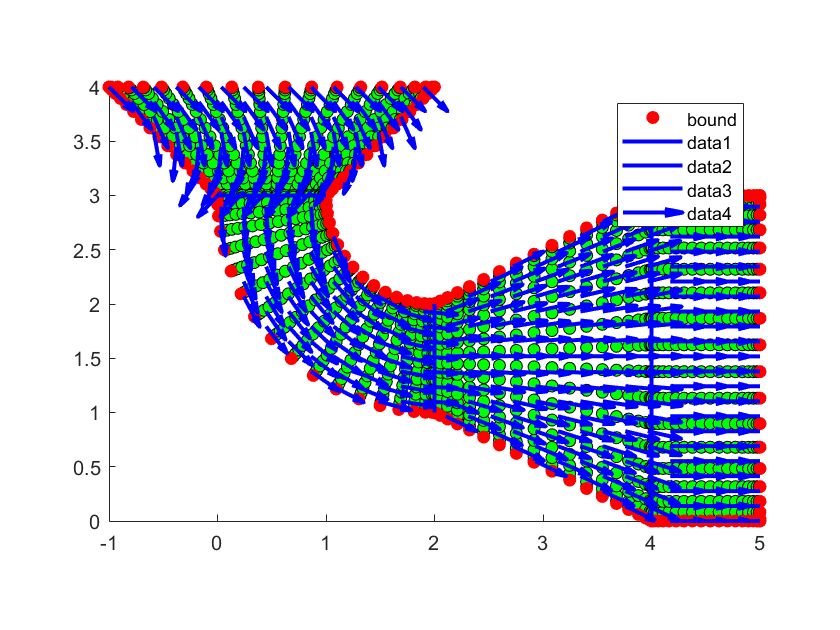
\includegraphics[scale=0.35]{F1.png}
%		\caption{Forward $\rho$ for $a = 0.01$} 
%		\label{F1}
%	\end{figure}

\begin{document}
	
	
	

\section{Varying External Potential}
(Note: MSSeparationOCP in code)
We consider the overdamped DDFT with no flux boundary conditions, a Gaussian pair potential and for the forward problem, no background flow. 
The external potential is given by
\begin{align*}
	V_{ext} =  \cos(2\pi (t + 0.5)/2.75)r^2,
\end{align*}
see Figure \ref{F1}. The time horizon for the problem is $(0,3)$ with $n = 30$ and the spatial domain is a box of dimension $[-5,5]^2$ with $N = 30$. The initial condition for $\rho$ is the uniform distribution $\rho_0 = 0.8$. The ODE tolerances are set to be $10^{-8}$. All figures show the time points $2,\  5,\ 8,\  10,\ 12,\ 14,\ 16,\ 18,\ 20,\ 23,\ 26$ out of $30$.
While Figure \ref{F0c} shows the effect of $V_{ext}$ in absence of the interaction term, Figures \ref{F0a} and \ref{F0b} show the effect of the positive and negative attraction term in absence of the external potential. We note that the change in $\rho$ by these interactions is of the same magnitude as the effect of $V_{ext}$. In Figures \ref{F2a} and \ref{F2b} the effects of $V_{ext}$ in combination with the two different interaction potentials are shown. Note that in Figure \ref{F2a} the maximum of the colour range is $\max \rho - 1.2$ in order to capture all important aspects of the dynamics over the time horizon. All other plots show the colour range $(\min \rho , \max \rho)$.\\
\\
These forward problems are now used in the context of an optimal control problem. We are interested in optimizing a system without external potential present to mimic those with the chosen external potential. Therefore, we first set $\hr$ to be the forward problem without particle interactions ($\kappa =0$) and with the external potential, see Figure \ref{F0c}. We then start the optimization by choosing the same uniform initial condition for $\rho$ but without an external potential. The intitial guess for $\w$ is zero. We then expect $\w$ to mimic the external potential, forcing particles in the desired state and it is of interest in what way this flow control is similar to the external potential that shaped $\hr$.
The same experiment is conducted with repulsive particles ($\kappa = 0.5$), where Figure \ref{F2a} shows the desired state and Figure \ref{F0a} displays the uncontrolled, initial state for the optimization. Then for attractive particles ($\kappa = -0.$) we have that $\hr$ takes the form shown in Figure \ref{F2b}, while the uncontrolled profile of $\rho$ is displayed in Figure \ref{F0b}.\\
\\
We choose $\lambda = 0.001$, since the problem is quite complex to solve and $\lambda = 0.01$ is an unstable choice.
\begin{figure}[h]
	\centering
	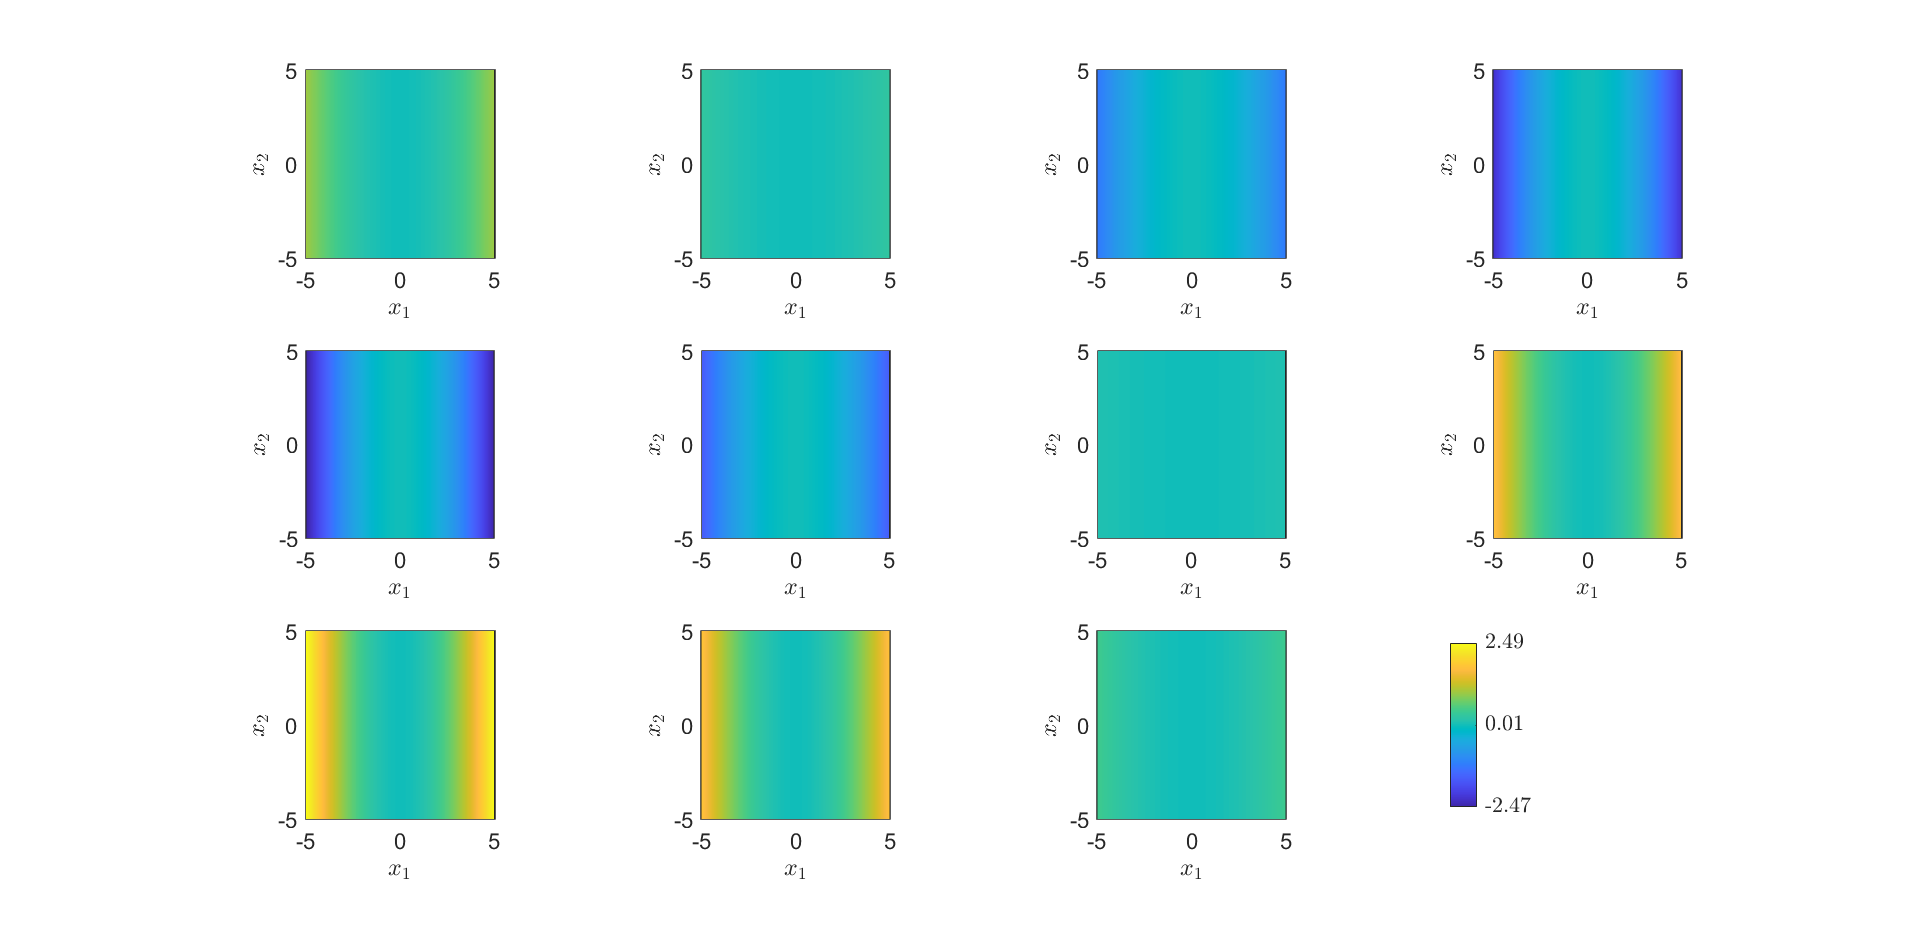
\includegraphics[scale=0.35]{Vext.png}
	\caption{External potential over time.} 
	\label{F1}
\end{figure}
\begin{figure}[h]
	\centering
	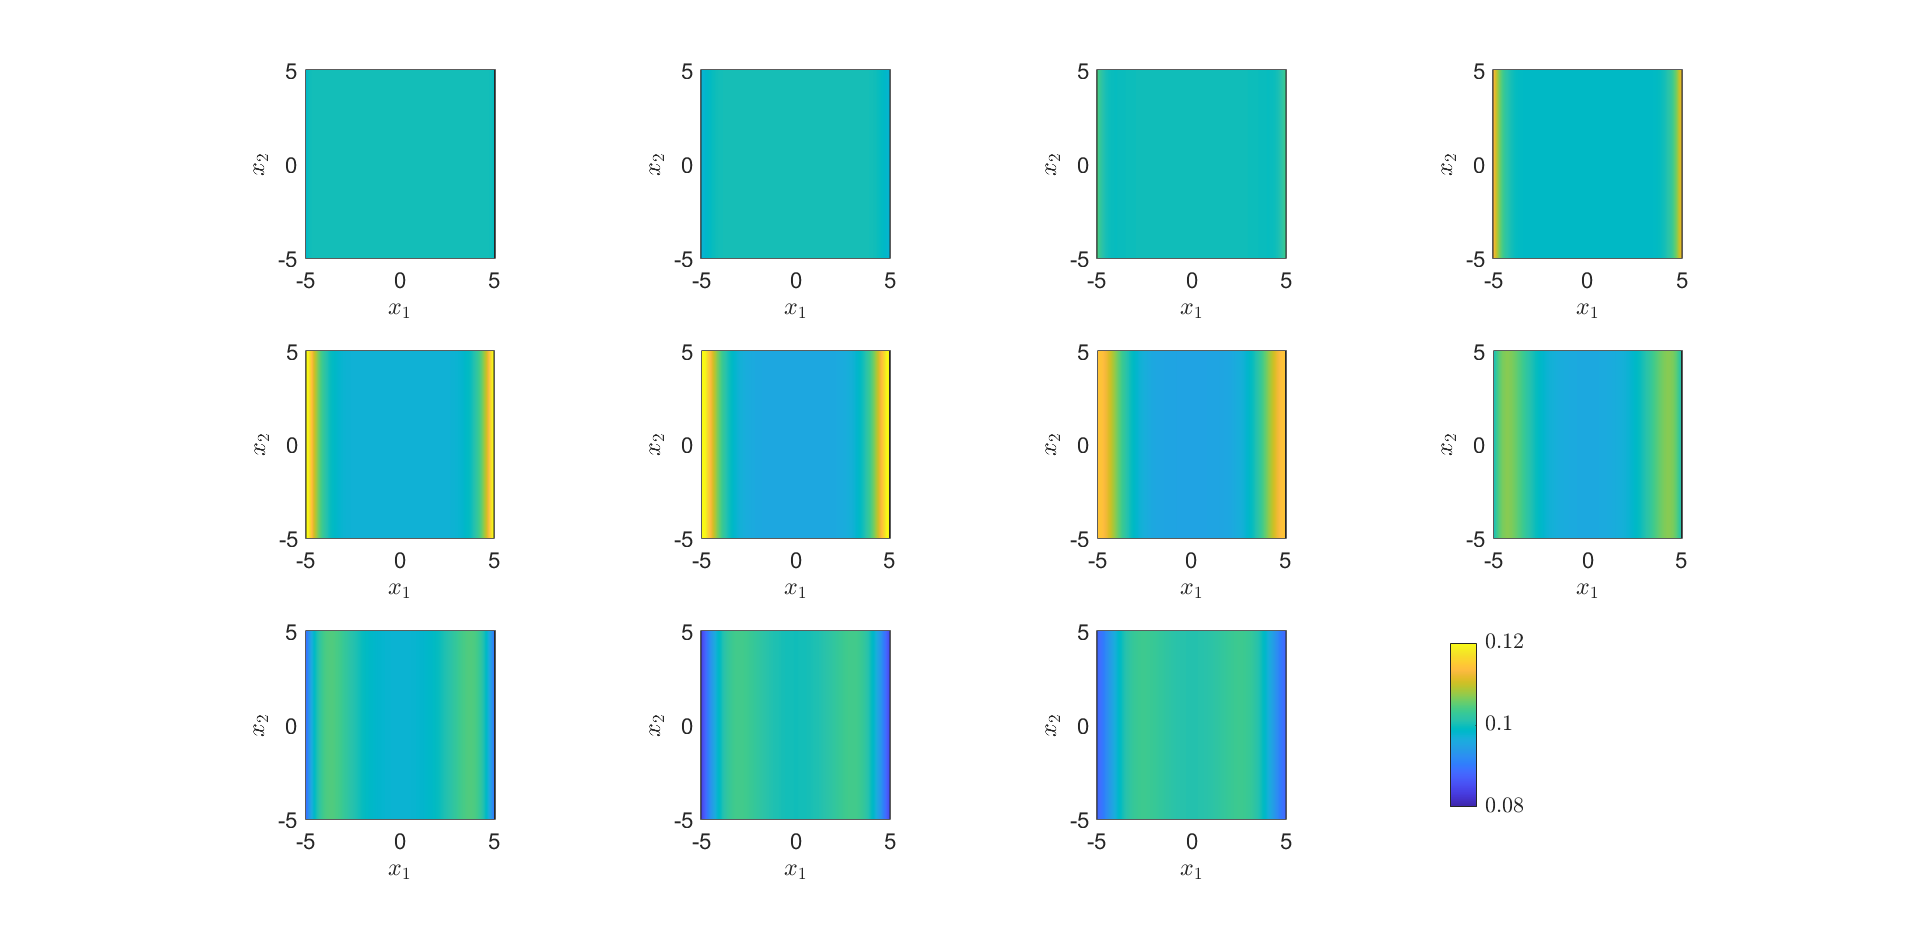
\includegraphics[scale=0.35]{rhok0V.png}
	\caption{Forward $\rho$ over time horizon, $\kappa = 0$, $V_{ext}$ on. This is the desired state $\hr$ for the uncontrolled particle distribution without interactions, which is a uniform distribution.} 
	\label{F0c}
\end{figure}
\begin{figure}[h]
	\centering
	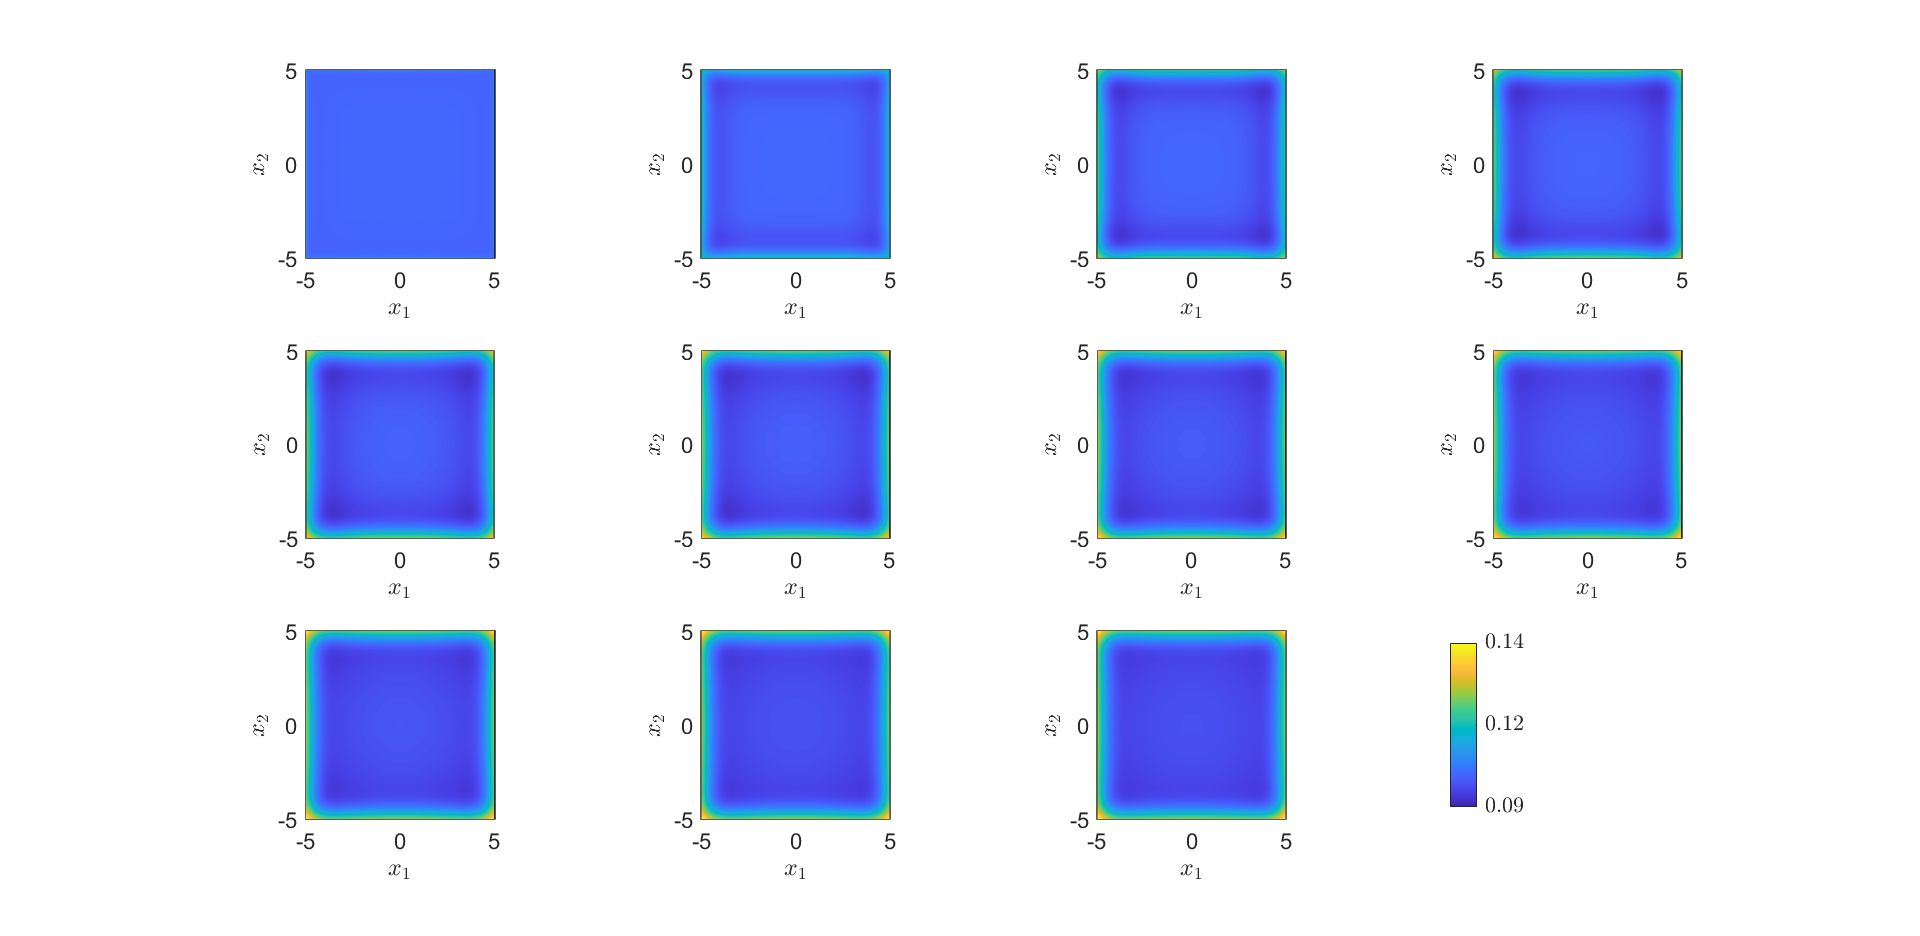
\includegraphics[scale=0.35]{rhok05.png}
	\caption{Forward $\rho$ over time horizon, $\kappa = 0.5$, $V_{ext}$ off. This is the uncontrolled state corresponding to the desired state $\hr$ displayed in Figure \ref{F2a}.} 
	\label{F0a}
\end{figure}
\begin{figure}[h]
	\centering
	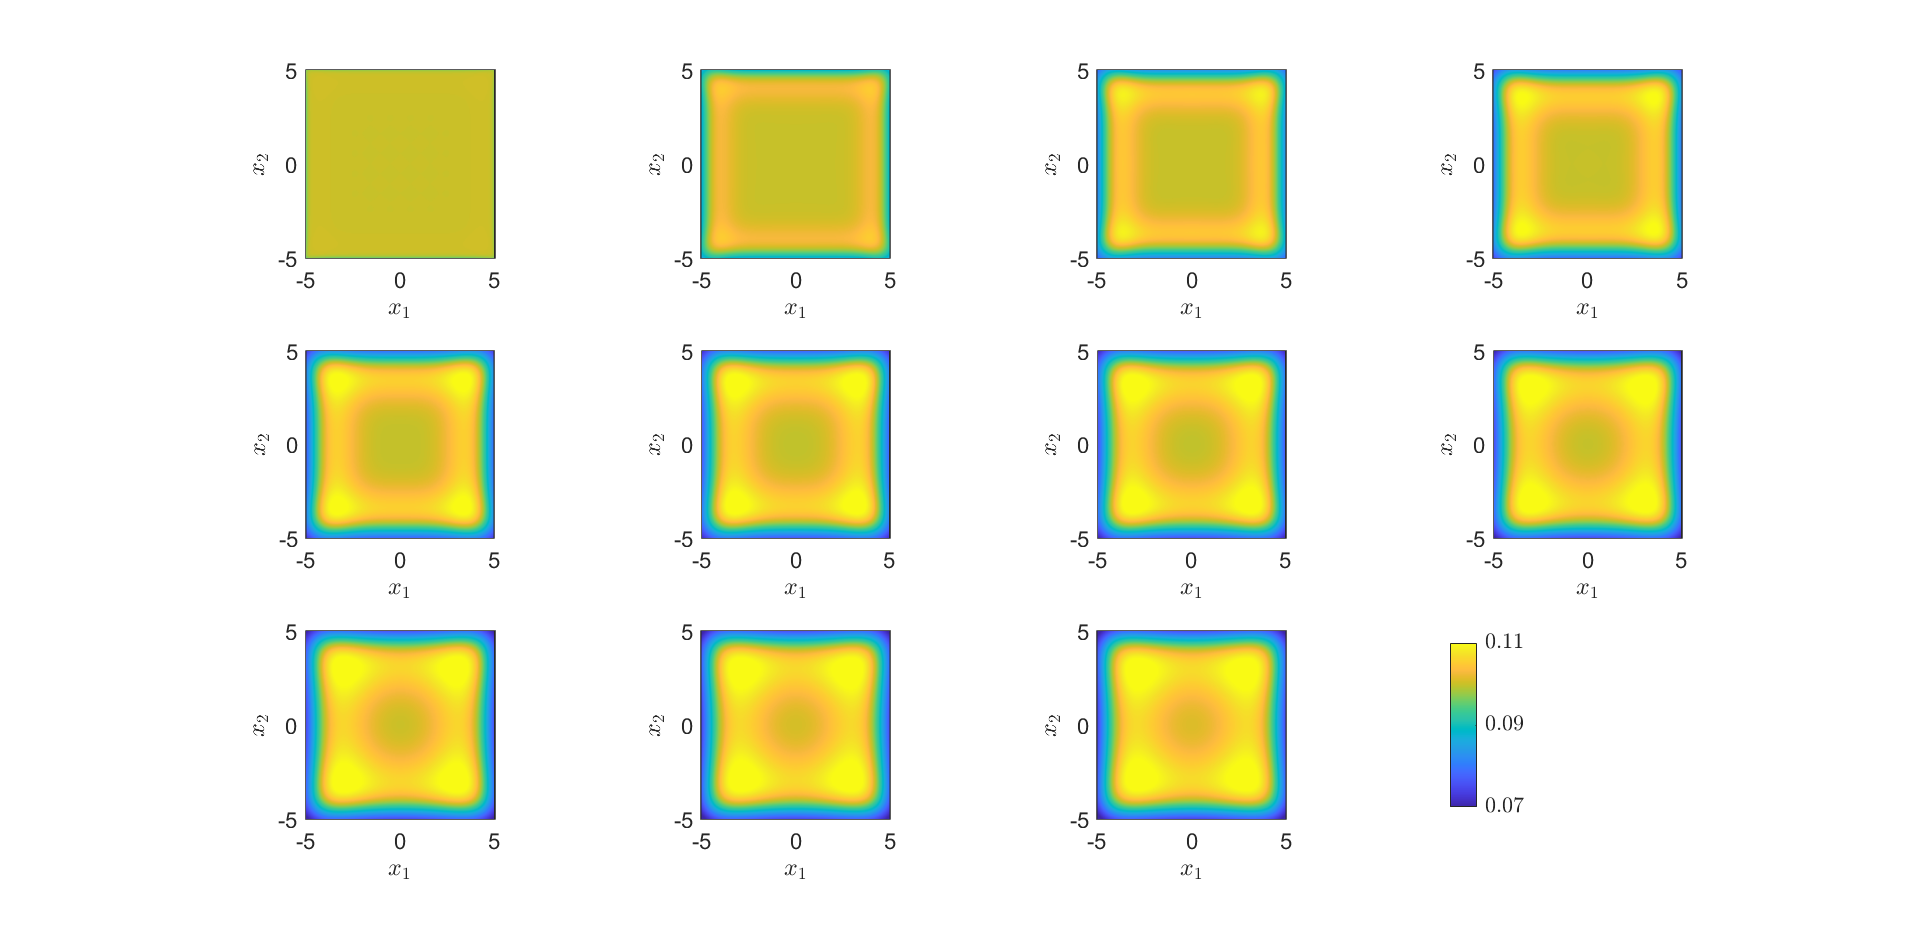
\includegraphics[scale=0.35]{rhokn05.png}
	\caption{Forward $\rho$ over time horizon, $\kappa = - 0.5$, $V_{ext}$ off. This is the uncontrolled state corresponding to the desired state $\hr$ displayed in Figure \ref{F2b}.} 
	\label{F0b}
\end{figure}



\begin{figure}[h]
	\centering
	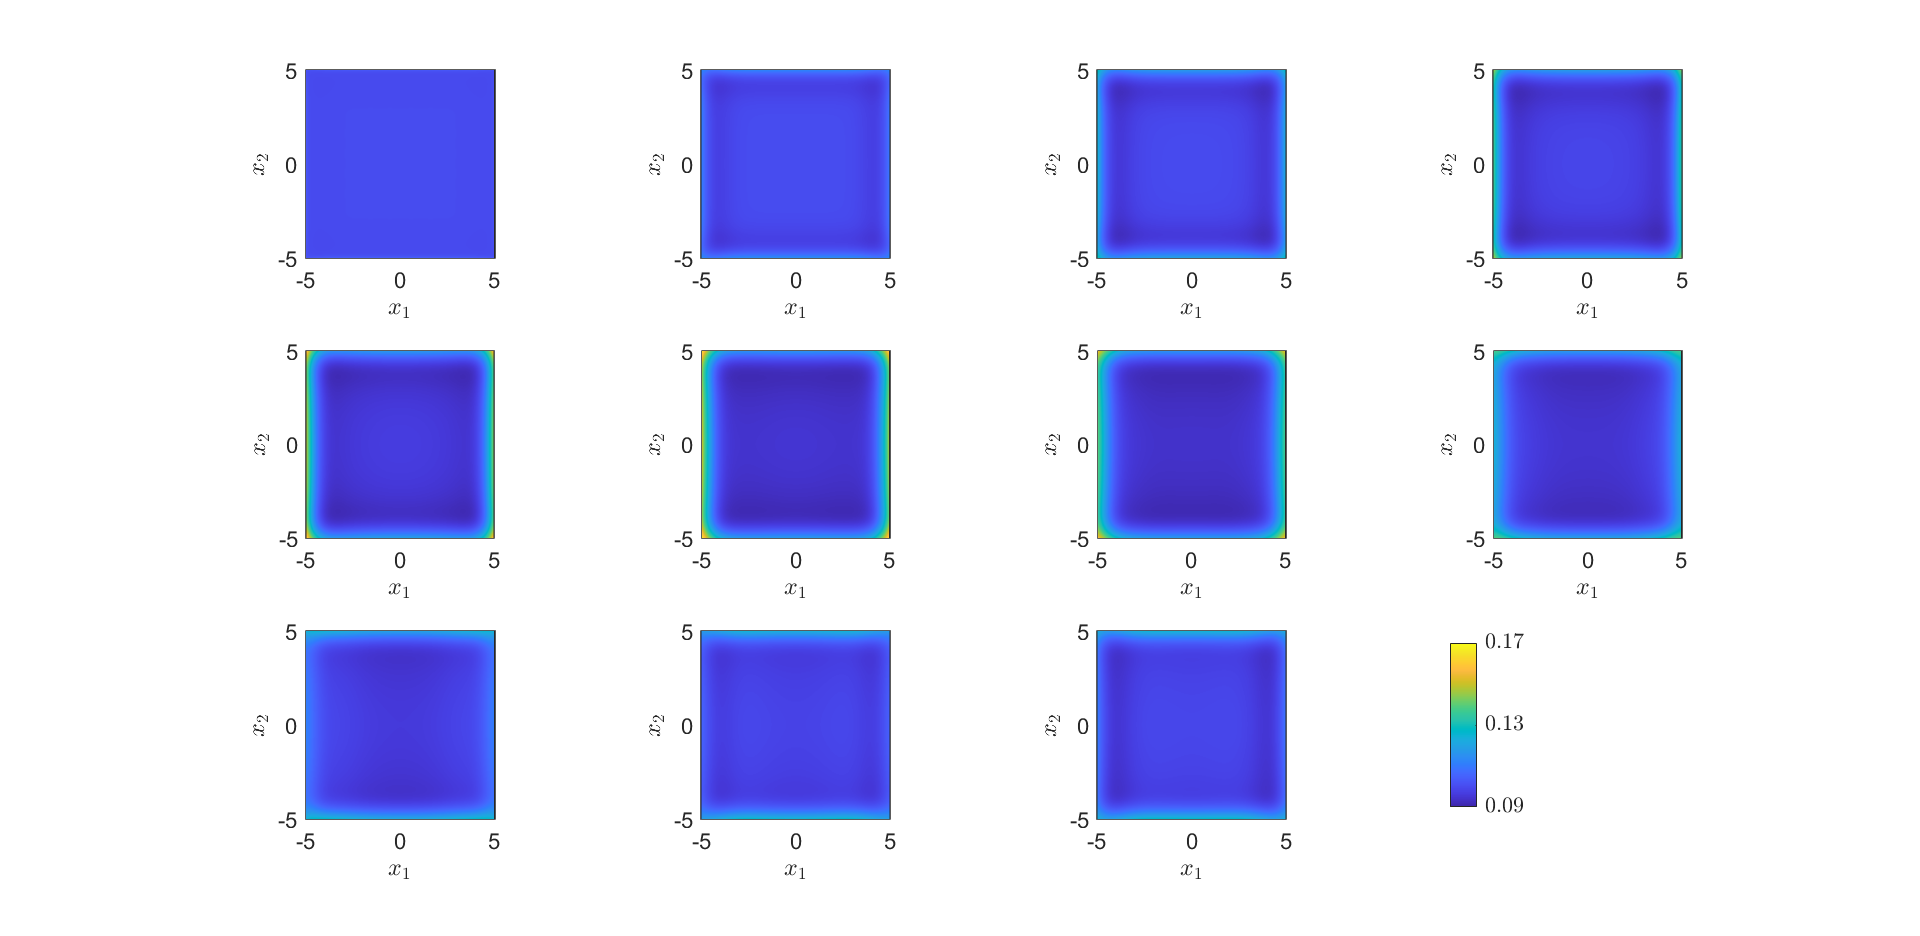
\includegraphics[scale=0.35]{rhok05V.png}
	\caption{Forward $\rho$ over time horizon, $\kappa = 0.5$, $V_{ext}$ on. Note that the colour range is from $\min \rho$ to $(\max \rho) - 1.2$ for illustratory purposes. This is the desired state $\hr$ for the uncontrolled particle distribution shown in Figure \ref{F0a}.} 
	\label{F2a}
\end{figure}
\begin{figure}[h]
	\centering
	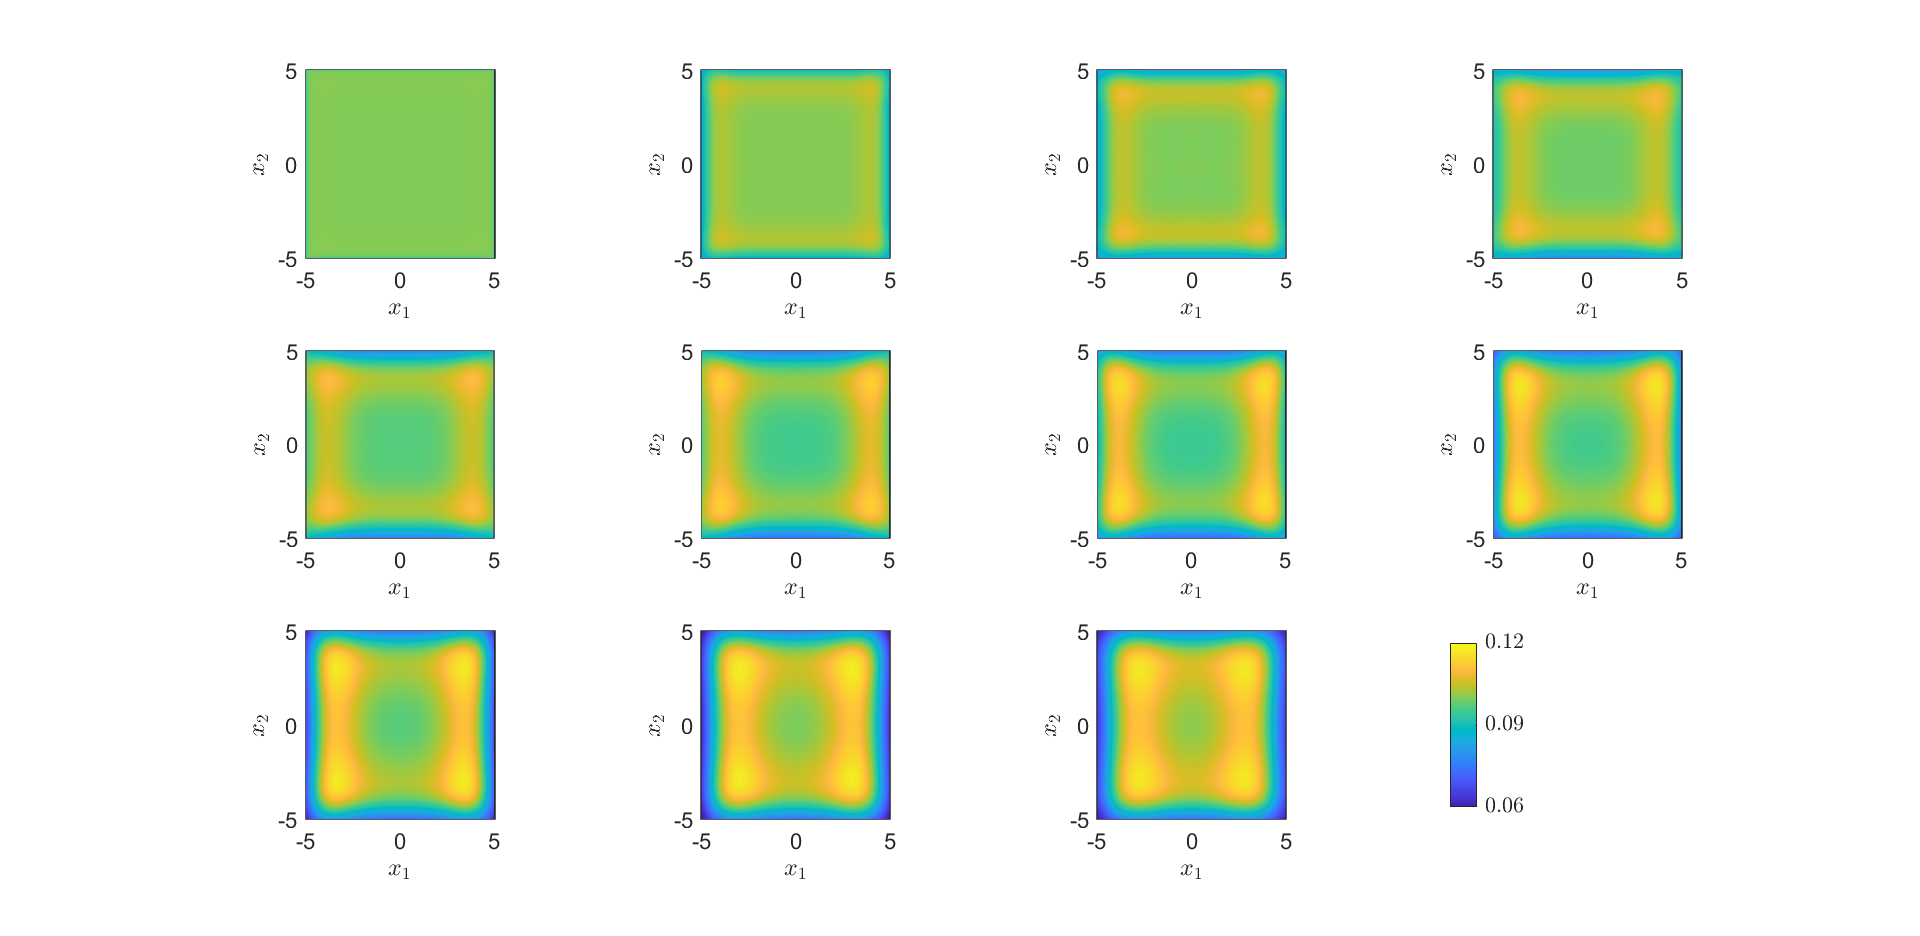
\includegraphics[scale=0.35]{rhokn05V.png}
	\caption{Forward $\rho$ over time horizon, $\kappa = - 0.5$, $V_{ext}$ on. This is the desired state $\hr$ for the uncontrolled particle distribution shown in Figure \ref{F0b}.} 
	\label{F2b}
\end{figure}





\end{document}